\documentclass[a4paper,9pt,twocolumn]{ltjsarticle}

\usepackage{midreport}
\usepackage{appendix}
\usepackage{newtxtext,newtxmath}
\usepackage{graphicx}
\graphicspath{{fig/}}

\setcounter{topnumber}{100}
\setcounter{totalnumber}{100}
\renewcommand{\topfraction}{0.67}
\renewcommand{\textfraction}{0.25}

\title{VR視覚刺激に対する立位姿勢応答を用いた\\視覚フィードバック特性の同定}
\etitle{Identification of Visual Feedback Characteristics Using Standing Postural Responses to VR Visual Stimuli}

\author{髙橋研究室 学部4年 瀬口 ことみ}
\eauthor{Kotomi SEGUCHI}

\affiliation{Keio University, 3-14-1 Hiyoshi, Kohoku-ku, Yokohama}

\fancyhead[L,R]{1-B4-4}
\fancyfoot[C]{%
  慶應義塾大学システムデザイン工学科\,
  髙橋研究室 第1回中間発表 2026/12/04\\
  -- \thepage\ --
}

\begin{document}

\twocolumn[
  \maketitle

  \begin{abstract}
    本研究では，Virtual Reality ( VR ) による視覚刺激に対する立位時の身体重心応答から，
    姿勢制御モデルの視覚フィードバック特性を同定する手法を検討する．
    支持面を固定したまま視覚外乱を独立に提示し，実測した周波数応答とモデル応答の比較により，
    視覚フィードバックの時定数およびゲインを推定する．
    さらに，同定結果の妥当性，識別可能性および試行間再現性を検証する．

    \textbf{\textit{Keywords}}: postural control, visual feedback, virtual reality, optic flow, system identification
  \end{abstract}
]

\section{緒言}

\subsection{研究背景}

ヒトは視覚，前庭感覚，体性感覚などの複数の感覚情報を統合することで
立位姿勢を維持している．
各感覚情報の寄与は一定ではなく，周囲の環境や身体の状態に応じて変化する．
Peterkaは，視覚刺激および支持面外乱に対する姿勢応答を解析し，
感覚情報の重み付けを含む姿勢制御モデルを提案した\cite{peterka2002}．

\subsubsection{転倒予防への応用}

高齢化に伴う転倒の予防には，この感覚統合特性を考慮した姿勢制御評価が重要である．
転倒外来を受診した高齢者では，視覚依存性がめまいや複数回の転倒と関連することが
報告されている\cite{barr2016}．
また，高齢者は若年者より姿勢制御における視覚寄与が高く\cite{neumann2025}，
動く視覚刺激に対して大きな姿勢動揺を示す傾向がある\cite{phu2023}．
一方，反復的なVR視覚刺激によって高齢者の視覚誘発性姿勢動揺が低減する
可能性も示されている\cite{barbanchon2026}．
VRを用いたバランス評価・訓練では，年齢や健康状態，個人の特性に応じた
刺激条件の設定が必要である\cite{soltani2021}．
したがって，視覚刺激に対する身体応答を定量化することは，
個人に適した転倒予防およびリハビリテーション設計につながる可能性がある．

\subsubsection{PPPDの評価への応用}

持続性知覚性姿勢誘発めまい ( Persistent Postural-Perceptual Dizziness: PPPD ) では，
立位，身体運動，動く視覚刺激または複雑な視覚環境への曝露によって，
めまいや不安定感が増加することが知られている\cite{staab2017}．
このようにPPPD患者には視覚刺激が主な増悪因子となる一群がある一方，
従来の前庭機能検査ではその特徴を十分に識別できないことが報告されている\cite{yagi2021}．
このため，視覚刺激に対する身体応答を客観的な指標で評価し，
個人ごとの視覚依存性を定量化する方法が求められる．

\subsection{従来研究}

Sonobe and Miuraは，支持面の水平動揺に対する身体重心 ( Center of Mass: COM ) の応答に着目し，人体を1リンク倒立振子として表現した姿勢制御モデルを提案した\cite{sonobe2025}．
同モデルは，時間遅れを含む状態フィードバック制御に加え，
支持面速度に応じてCOMの目標位置が変化する機構を備える．
この機構を視覚フィードバックの影響と仮定し，その時定数およびゲインを同定している．

しかし，支持面を動揺させる従来手法では，
身体への力学的外乱と視覚的外乱が同時に生じるため，
視覚情報の影響を独立して評価することが難しい．
また，同研究の級内相関係数 ( Intraclass Correlation Coefficient: ICC ) は，
視覚フィードバックの時定数$T_v$についてDay 1--Day 2で0.142，
Day 2--Day 3で0.642，Day 1--Day 3で0.290であった\cite{sonobe2025}．
ゲイン$\gamma_v$のICCはそれぞれ0.691，0.642，0.494であり，
特に$T_v$の試行日間再現性には改善の余地がある．

\subsection{課題解決のアプローチ}

そこで本研究では，支持面を固定した状態で視覚外乱のみを提示できるVRに着目する．
VR空間の前後運動を入力，立位時のCOM動揺を出力として周波数応答を求め，
実測応答と姿勢制御モデルの応答が一致するように視覚フィードバックパラメータを同定する．
一方，支持面外乱を前提とした従来モデルをVR視覚刺激へ適用するには，
モデル入力の定義および伝達関数の構造を再検討する必要がある．

\subsection{研究の独創性}

本研究の独創性は，力学的外乱を伴う支持面動揺ではなく，
支持面を固定したVR環境で視覚外乱を独立に与える点にある．
これにより，視覚情報がCOM目標位置へ反映される時間特性$T_v$と，
視覚刺激に対する姿勢の影響されやすさを表すゲイン$\gamma_v$を分離して評価する．
さらに，同定値を提示するだけでなく，ICCによる再現性評価と正規化感度係数による
固定パラメータの妥当性評価を組み合わせ，臨床評価や介入効果の検証に利用可能な指標を目指す．

\section{研究概要}

\subsection{研究目的}

本研究の目的は，VR視覚刺激に対する立位時のCOM応答から，
姿勢制御モデルにおける視覚フィードバック特性を同定する手法を構築することである．
身体および姿勢制御に関するパラメータを固定し，
視覚フィードバックの時定数$T_v$とゲイン$\gamma_v$を同定する．
さらに，実測応答とモデル応答を比較し，モデルの妥当性，
パラメータの識別可能性および試行間再現性を検証する．

\section{立位姿勢制御モデル}

\subsection{モデルの概要}

本研究では，Sonobe and Miuraのモデル\cite{sonobe2025}を基礎とする．
人体を足関節まわりに回転する1リンク倒立振子として近似し，
姿勢制御を比例・微分 ( PD ) 制御および時間遅れを含むフィードバック系として表現する．
園部らは，支持面加速度に対してCOM応答の位相が0.3\,Hz以下で約90度進む特徴に着目し，
視覚で知覚した支持面速度に身体が引き込まれることでCOM平衡位置が移動する，
という仮説を一次遅れ系としてモデル化した\cite{sonobe2025}．
これは一般的な低周波補償として積分項を導入したものではなく，
視覚刺激に対する低周波応答を説明するための仮説である．

身体重心の水平変位を$x_b$，支持面変位を$X_s$，
足関節まわりの制御トルクを$N_a$とすると，運動方程式は

\begin{equation}
  (\frac{J_b}{l_b}+m_b l_b)\ddot{x}_b(t)-m_b g x_b(t)
  =-m_b l_b\ddot{X}_s(t)+N_a(t)
  \label{eq:motion}
\end{equation}

と表される．ここで，$m_b$，$J_b$，$l_b$はそれぞれ身体の質量，
足関節まわりの慣性モーメント，足関節から身体重心までの距離である．
制御トルクは，時間遅れ$t_d$を含むPD制御として

\begin{equation}
  N_a(t)=-k_p\left\{x_b(t-t_d)-\bar{x}_b(t-t_d)\right\}
  -k_d\dot{x}_b(t-t_d)
  \label{eq:torque}
\end{equation}

とする．目標重心位置$\bar{x}_b$は，
視覚フィードバックの時定数$T_v$とゲイン$\gamma_v$を用いて

\begin{equation}
  T_v\dot{\bar{x}}_b(t)+\bar{x}_b(t)=-\gamma_v\dot{X}_s(t)
  \label{eq:visual-feedback}
\end{equation}

と表される．
本研究では，式\eqref{eq:motion}および式\eqref{eq:torque}の身体・制御パラメータを
既知とし，VR視覚刺激に対する応答から
式\eqref{eq:visual-feedback}の$T_v$と$\gamma_v$を同定する．
ただし，従来研究とは外乱の提示方法が異なるため，
$X_s$をVR空間の運動へ読み替えたときの入力定義と伝達関数の構造を検討する．
モデルの概略図をFig.~\ref{fig:model}に示す．
%「既知とし」の部分に具体的な説明が欲しい（後述してるからいらないか？）

\suppressfloats[t]
\begin{figure}[t]
  \centering
  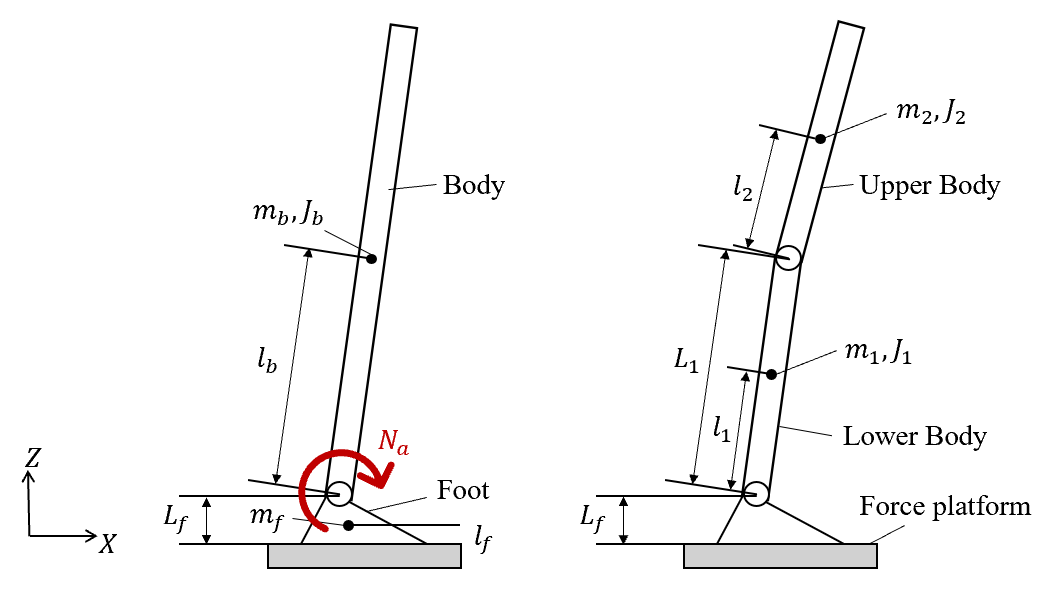
\includegraphics[width=0.88\columnwidth]{sonobe2025_fig2_re.png}
  \caption{Mechanical models for estimating COM displacement: ( a ) single inverted pendulum and ( b ) double inverted pendulum models}
  \label{fig:model}
\end{figure}

\subsection{同定対象および固定パラメータ}

同定対象は，視覚刺激に対する応答の時間特性を表す時定数$T_v$と，
視覚刺激が姿勢制御へ及ぼす影響の大きさを表すゲイン$\gamma_v$である．
$T_v$は視覚刺激の変化がCOM目標位置へ反映される速さを表すため，
介入や反復提示の前後で視覚応答の時間特性が変化したかを検証する指標となる．
$\gamma_v$は視覚運動に対してCOM目標位置がどの程度移動するかを表し，
視覚刺激に対する姿勢の影響されやすさを定量化する指標となる．

同定対象を2パラメータに限定するため，
身体質量，重心位置，慣性モーメントなどの身体パラメータ，
PD制御ゲインおよび制御時間遅れは先行研究を参考に固定する．
身体パラメータは体重$M$と身長$H$からTable~\ref{tab:physical-parameters}の近似式で算出する．

\begin{equation}
  K_p=\frac{k_p}{J_b/l_b+m_b l_b},\qquad
  K_d=\frac{k_d}{J_b/l_b+m_b l_b}
  \label{eq:normalized-gains}
\end{equation}

式\eqref{eq:normalized-gains}の正規化ゲインを用いることで，
体型差を考慮して制御ゲインを設定できる．
支持面を物理的に並進させた園部らの条件では，力学的外乱と視覚外乱が同時に作用するため，
そこで得られたPDゲインと遅延をVR視覚外乱のみの本実験へ直接適用することは妥当でない可能性がある．
そこで，VR内の視覚シーンを動揺させたAssl\"anderらの実験を固定値の根拠とする\cite{asslaender2023}．
同研究の短時間PRTS条件における代表値
$\widetilde{K}_p\simeq1.27$，$\widetilde{K}_d\simeq0.46\,\mathrm{s}$，
$t_d\simeq0.18\,\mathrm{s}$を候補とする．
ここで$\widetilde{K}_p$および$\widetilde{K}_d$は$m_b g l_b$で正規化された角度入力のゲインである．
Assl\"anderらの角度表現をラジアンへ統一した後，
小角近似$x_b=l_b\theta$を用いて本研究の並進変位入力へ換算すると

\begin{equation}
  k_p=\widetilde{K}_p m_b g,\qquad
  k_d=\widetilde{K}_d m_b g
  \label{eq:gain-conversion}
\end{equation}

として単位を換算した後，式\eqref{eq:normalized-gains}の$K_p$および$K_d$へ変換する．
Assl\"anderらは日内3試行を平均した日間比較で，$K_p$，$K_d$，$t_d$に対して
それぞれICC=0.87，0.92，0.77を報告しており，固定値候補として一定の再現性を有する\cite{asslaender2023}．
なお，固定パラメータの選択が$T_v$および$\gamma_v$へ与える影響は，
正規化感度係数を用いて確認する．

\suppressfloats[t]
\begin{table}[t]
  \centering
  \caption{Physical parameters estimated from body mass $M$ and height $H$}
  \label{tab:physical-parameters}
  \footnotesize
  \setlength{\tabcolsep}{3.5pt}
  \begin{tabular}{@{}llcc@{}}
    \hline
    Segment & Symbol & Male & Female \\
    \hline
    Body & $m_b$ & $0.978M$ & $0.978M$ \\
         & $J_b$ & $0.0425MH^2$ & $0.0441MH^2$ \\
         & $l_b$ & $0.531H$ & $0.523H$ \\
    \hline
    Lower body & $m_1$ & $0.322M$ & $0.352M$ \\
         & $J_1$ & $0.00223MH^2$ & $0.00249MH^2$ \\
         & $l_1$ & $0.285H$ & $0.291H$ \\
         & $L_1$ & $0.460H$ & $0.460H$ \\
    \hline
    Upper body & $m_2$ & $0.656M$ & $0.626M$ \\
         & $J_2$ & $0.0114MH^2$ & $0.0121MH^2$ \\
         & $l_2$ & $0.191H$ & $0.193H$ \\
    \hline
    Foot & $m_f$ & $0.022M$ & $0.022M$ \\
         & $l_f$ & $0.015H$ & $0.015H$ \\
         & $L_f$ & $0.038H$ & $0.038H$ \\
    \hline
  \end{tabular}
\end{table}

\section{実験方法}

\subsection{実験システム}

被験者はヘッドマウントディスプレイMeta Quest 3 ( Meta Platforms Technologies, USA ) を装着し，床反力計上で静止立位を保持する．VR空間内の視覚環境を前後方向へ移動させることで，支持面を固定したまま視覚外乱を提示する．床反力およびモーメントから前後方向のCOM変位を推定し，補助計測として頭部に慣性計測装置 ( IMU ) を装着する．刺激提示PCには視覚刺激の時刻および運動情報を記録し，床反力計のデータと時間同期する．実験システムの概略図をFig.~\ref{fig:system}に示す．

\suppressfloats[t]
\begin{figure}[t]
  \centering
  
\includegraphics[width=0.88\columnwidth]{sample.jpg}
  \caption{Placeholder for the experimental system}
  \label{fig:system}
\end{figure}

\subsection{VR視覚刺激}

VR空間には格子状の視覚環境を構築し，その前後並進運動によって視覚刺激を与える．
提示するVR映像の例をFig.~\ref{fig:vr-scene}に示す．
姿勢制御系の周波数特性を評価するため，複数の周波数成分を含むマルチコサイン波と，
周波数を連続的に変化させるスイープ波を刺激候補として比較している．
刺激形式は今後確定するが，低周波数成分を陽に励起するため，
各周波数成分の加速度振幅は一定とする方針である．

加速度振幅を一定にすると，低周波数ほど速度振幅および変位振幅が大きくなり，
一定速度振幅の刺激よりも低周波数帯へ大きな刺激エネルギーを配分できる\cite{sonobe2025}．
刺激波形の例をFig.~\ref{fig:stimulus-waveform}に示す．
床反力計の制約から1試行を90秒とし，低周波数成分の解析精度を考慮して刺激を設計する．

\suppressfloats[t]
\begin{figure}[t]
  \centering
  
\includegraphics[width=0.88\columnwidth]{sample.jpg}
  \caption{Placeholder for the visual scene presented in VR}
  \label{fig:vr-scene}
\end{figure}

\suppressfloats[t]
\begin{figure}[t]
  \centering
  
\includegraphics[width=0.88\columnwidth]{sample.jpg}
  \caption{Placeholder for the visual stimulus waveform}
  \label{fig:stimulus-waveform}
\end{figure}

\section{解析方法}

\subsection{COM変位の推定と周波数応答解析}

床反力計から得たデータに必要な前処理を施し，視覚刺激入力と前後方向COM応答の時系列を取得する．低周波数帯を解析対象とするため，フィルタ処理によって対象成分が減衰しないようにする．

VR視覚刺激を入力，COM応答を出力として周波数応答関数 ( Frequency Response Function: FRF ) を算出し，ゲインおよび位相の周波数依存性を評価する．入力については刺激の変位，速度および加速度，出力についてはCOMの変位，速度および加速度を候補とし，物理的整合性，信号強度およびノイズの影響を比較する．

\subsection{パラメータ同定}

実測FRFとモデルFRFの複素誤差を最小化することで，$T_v$および$\gamma_v$を推定する．
現段階の予備同定では，$N_f$個の解析周波数$f_k$に対して

\begin{equation}
  \min_{T_v,\gamma_v} J
  =\sum_{k=1}^{N_f}w_k
  \left|
  \frac{H_{\mathrm{exp}}(f_k)-H_{\mathrm{mod}}(f_k;T_v,\gamma_v)}
  {H_{\mathrm{exp}}(f_k)}
  \right|^2
  \label{eq:objective}
\end{equation}

を非線形最小二乗法で解く．ここで$w_k$は各周波数のコヒーレンスに基づく重みである．
複素FRFを直接用いることで，ゲインと位相を同時に評価する．
探索範囲は現時点で$0.1\leq T_v\leq10\,\mathrm{s}$，
$0\leq\gamma_v\leq0.10\,\mathrm{s}$とし，境界値への収束の有無を確認しながら更新する．
両パラメータが独立かつ安定に推定可能かは，目的関数分布および感度解析により検証する．

\subsection{妥当性および再現性の検証}

同定したパラメータを用いてモデル応答を算出し，実測応答との比較からモデルの妥当性を評価する．
さらに，同一被験者の複数試行で得た$T_v$および$\gamma_v$についてICCを算出し，
試行間および日間再現性を評価する．
固定した$K_p$，$K_d$，$t_d$を基準値から変化させたときの
$T_v$および$\gamma_v$の正規化感度係数を求め，
感度が大きい固定パラメータについては固定値の再検討または同定対象への追加を判断する．
再現性が不十分な場合は，刺激の反復数，計測時間および同定方法を再検討する．

\section{予備実験}

\subsection{計測および解析の進捗}

健常者2名を対象とし，各2試行の予備実験を実施した．
1試行の計測時間は90秒とし，床反力計および頭部IMUによる計測を行った．
現在までに，刺激信号と床反力データの同期，COM変位の推定，
FRFの算出および式\eqref{eq:objective}に基づくパラメータ同定処理を実装した．
取得データでは視覚刺激の周波数に対応する身体応答成分を確認している．
周波数解析結果をFig.~\ref{fig:preliminary}に示す．

\suppressfloats[t]
\begin{figure}[t]
  \centering
  
\includegraphics[width=0.88\columnwidth]{sample.jpg}
  \caption{Placeholder for the frequency analysis results}
  \label{fig:preliminary}
\end{figure}

\subsection{同定条件}

予備同定では，以下に示す探索範囲を設定し，
複数の初期値から式\eqref{eq:objective}を最小化する．
解が探索境界に集中する場合は，探索範囲またはモデル構造が不適切である可能性を検討する．

\begin{center}
\begin{minipage}{0.9\columnwidth}
  \centering
  \textbf{Current constraints for preliminary identification}\\[2pt]
  \footnotesize
  \setlength{\tabcolsep}{5pt}
  \begin{tabular}{@{}lccc@{}}
    \hline
    Parameter & Lower & Upper & Unit \\
    \hline
    $T_v$ & 0.1 & 10 & s \\
    $\gamma_v$ & 0 & 0.10 & s \\
    \hline
  \end{tabular}
\end{minipage}
\end{center}

\subsection{予備同定結果}

各試行の同定結果を以下の表に整理する．
現段階では，低周波数帯の信号強度，初期値依存性および探索境界への収束を確認中である．
最終値は刺激形式と固定パラメータの確定後に更新する．

\begin{center}
\begin{minipage}{0.9\columnwidth}
  \centering
  \textbf{Provisional preliminary identification results}\\[2pt]
  \footnotesize
  \setlength{\tabcolsep}{4pt}
  \begin{tabular}{@{}lccc@{}}
    \hline
    Data & $T_v$ / s & $\gamma_v$ / s & $J$ \\
    \hline
    Subject 1, Trial 1 & -- & -- & -- \\
    Subject 1, Trial 2 & -- & -- & -- \\
    Subject 2, Trial 1 & -- & -- & -- \\
    Subject 2, Trial 2 & -- & -- & -- \\
    \hline
  \end{tabular}
\end{minipage}
\end{center}

\section{検討課題と今後の予定}

現在，VR刺激提示，計測データの同期，COM推定，FRF算出および
$T_v$，$\gamma_v$の予備同定までを実装している．
今後の主な検討課題は，以下の4点である．

\begin{enumerate}
  \item マルチコサイン波とスイープ波の比較および最終刺激形式の決定
  \item 加速度振幅一定条件における低周波数帯の信号強度と90秒試行の妥当性確認
  \item 固定パラメータに対する正規化感度係数の算出と固定値の確定
  \item $T_v$および$\gamma_v$の識別可能性，モデル適合度およびICCによる再現性の検証
\end{enumerate}

まず，予備実験データを用いて刺激形式，解析周波数帯および探索範囲を確定する．
次に，Assl\"anderらの値から換算した固定パラメータを基準として正規化感度係数を算出し，
固定の妥当性を確認する．その後，追加計測によって同定値のICCを算出し，
必要な試行数および平均化回数を決定する．
最終的に，介入または反復提示前後の$T_v$の変化と，
視覚刺激への影響されやすさを表す$\gamma_v$を用いて，
視覚フィードバック特性を定量評価できるかを検証する．

\section{結言}

本報告では，VR視覚刺激に対する立位時のCOM応答から，
視覚フィードバックの時定数とゲインを同定する手法を構築した．
予備実験では刺激周波数に対応する身体応答を確認し，
COM推定，FRF算出およびパラメータ同定までの解析処理を実装した．
今後は刺激形式と固定パラメータを確定し，正規化感度係数，モデル適合度およびICCを用いて，
パラメータの識別可能性，妥当性および再現性を検証する．

\bibliographystyle{IEEEtran}
\bibliography{bib}

\end{document}
